\documentclass[russian,utf8,a1paper,nostitching,simple]{eskdgraph}
\usepackage[T2A]{fontenc}
\usepackage{pscyr}
\usepackage{tikz}
\usepackage{color}

\newcommand{\No}{\textnumero}

\ESKDunitName{Калссы пользовательского интерфейса}
\ESKDsignature{ГУИР.000000.002 ПЛ}
\ESKDletter{}{Т}{}
\ESKDauthor{Будный}
\ESKDchecker{Лаппо}
\ESKDcolumnXIfIII{\color{red}{???}}
\ESKDnormContr{\color{red}{???}}
\ESKDapprovedBy{Навроцкий}
\ESKDgroup{ИТАС, гр. 120602}

\begin{document}

\ESKDthisStyle{empty}
\begin{ESKDdrawing}
  \begin{minipage}{.67\linewidth}
    \centering
    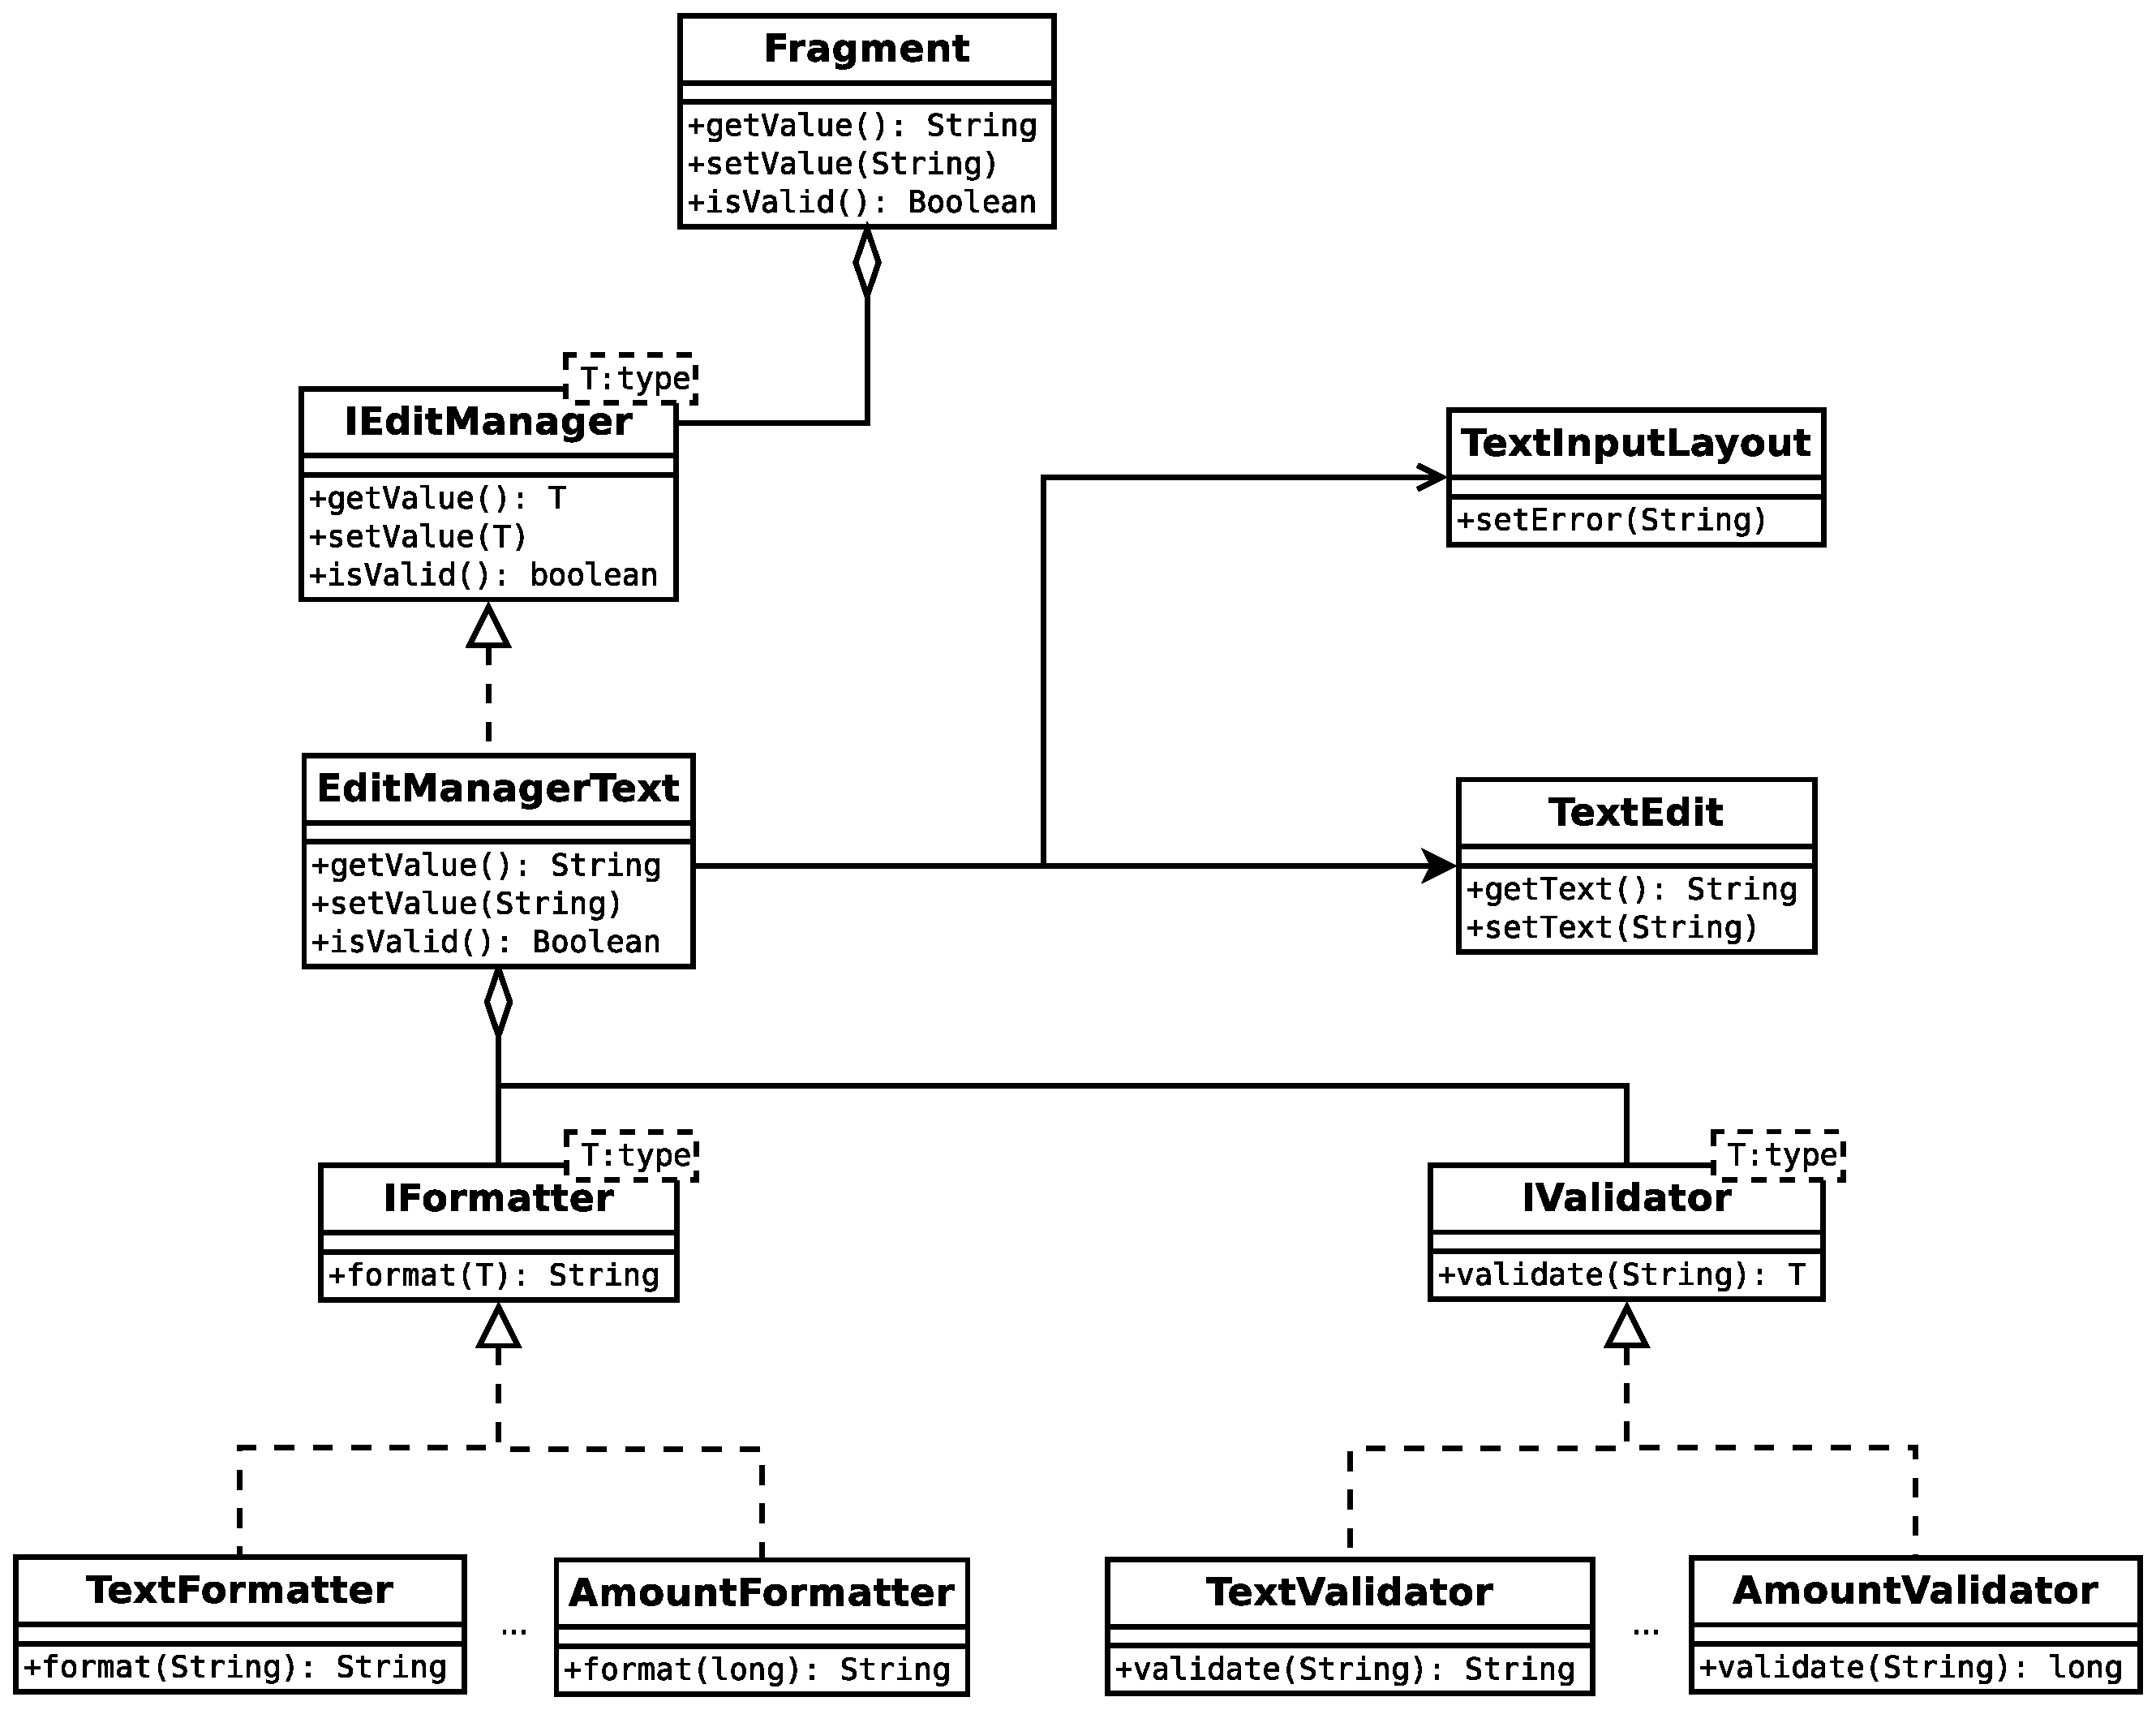
\includegraphics[height=44cm]{fig/implementation_ui_edit_manager.eps}

    \vspace{2cm}
    {\Huge{Диаграмма классов обработки данных, вводимых пользователем}}
  \end{minipage}
  \hspace{4cm}
  \begin{minipage}{0.25\linewidth}
    \centering
    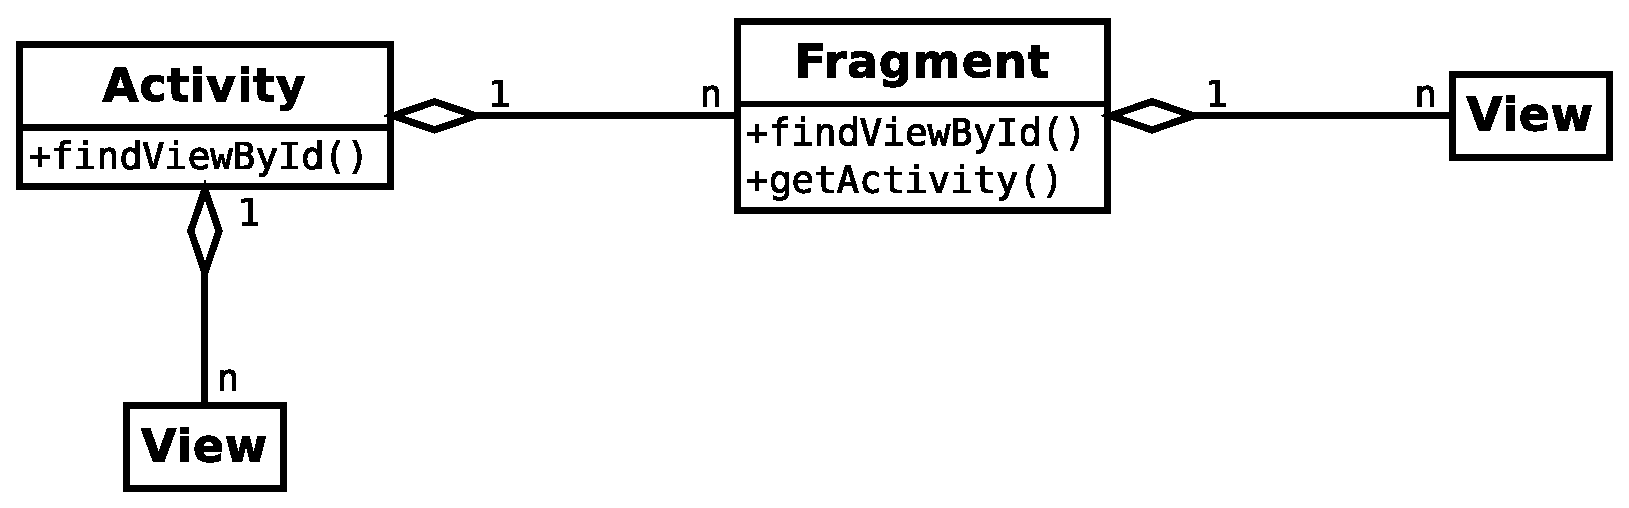
\includegraphics[height=6cm]{fig/implementation_ui_hierarchy.eps}

    \vspace{2cm}
    {\Huge{Иерархия базовых классов пользовательског интерфейса}}

    \vspace{4cm}
    \centering
    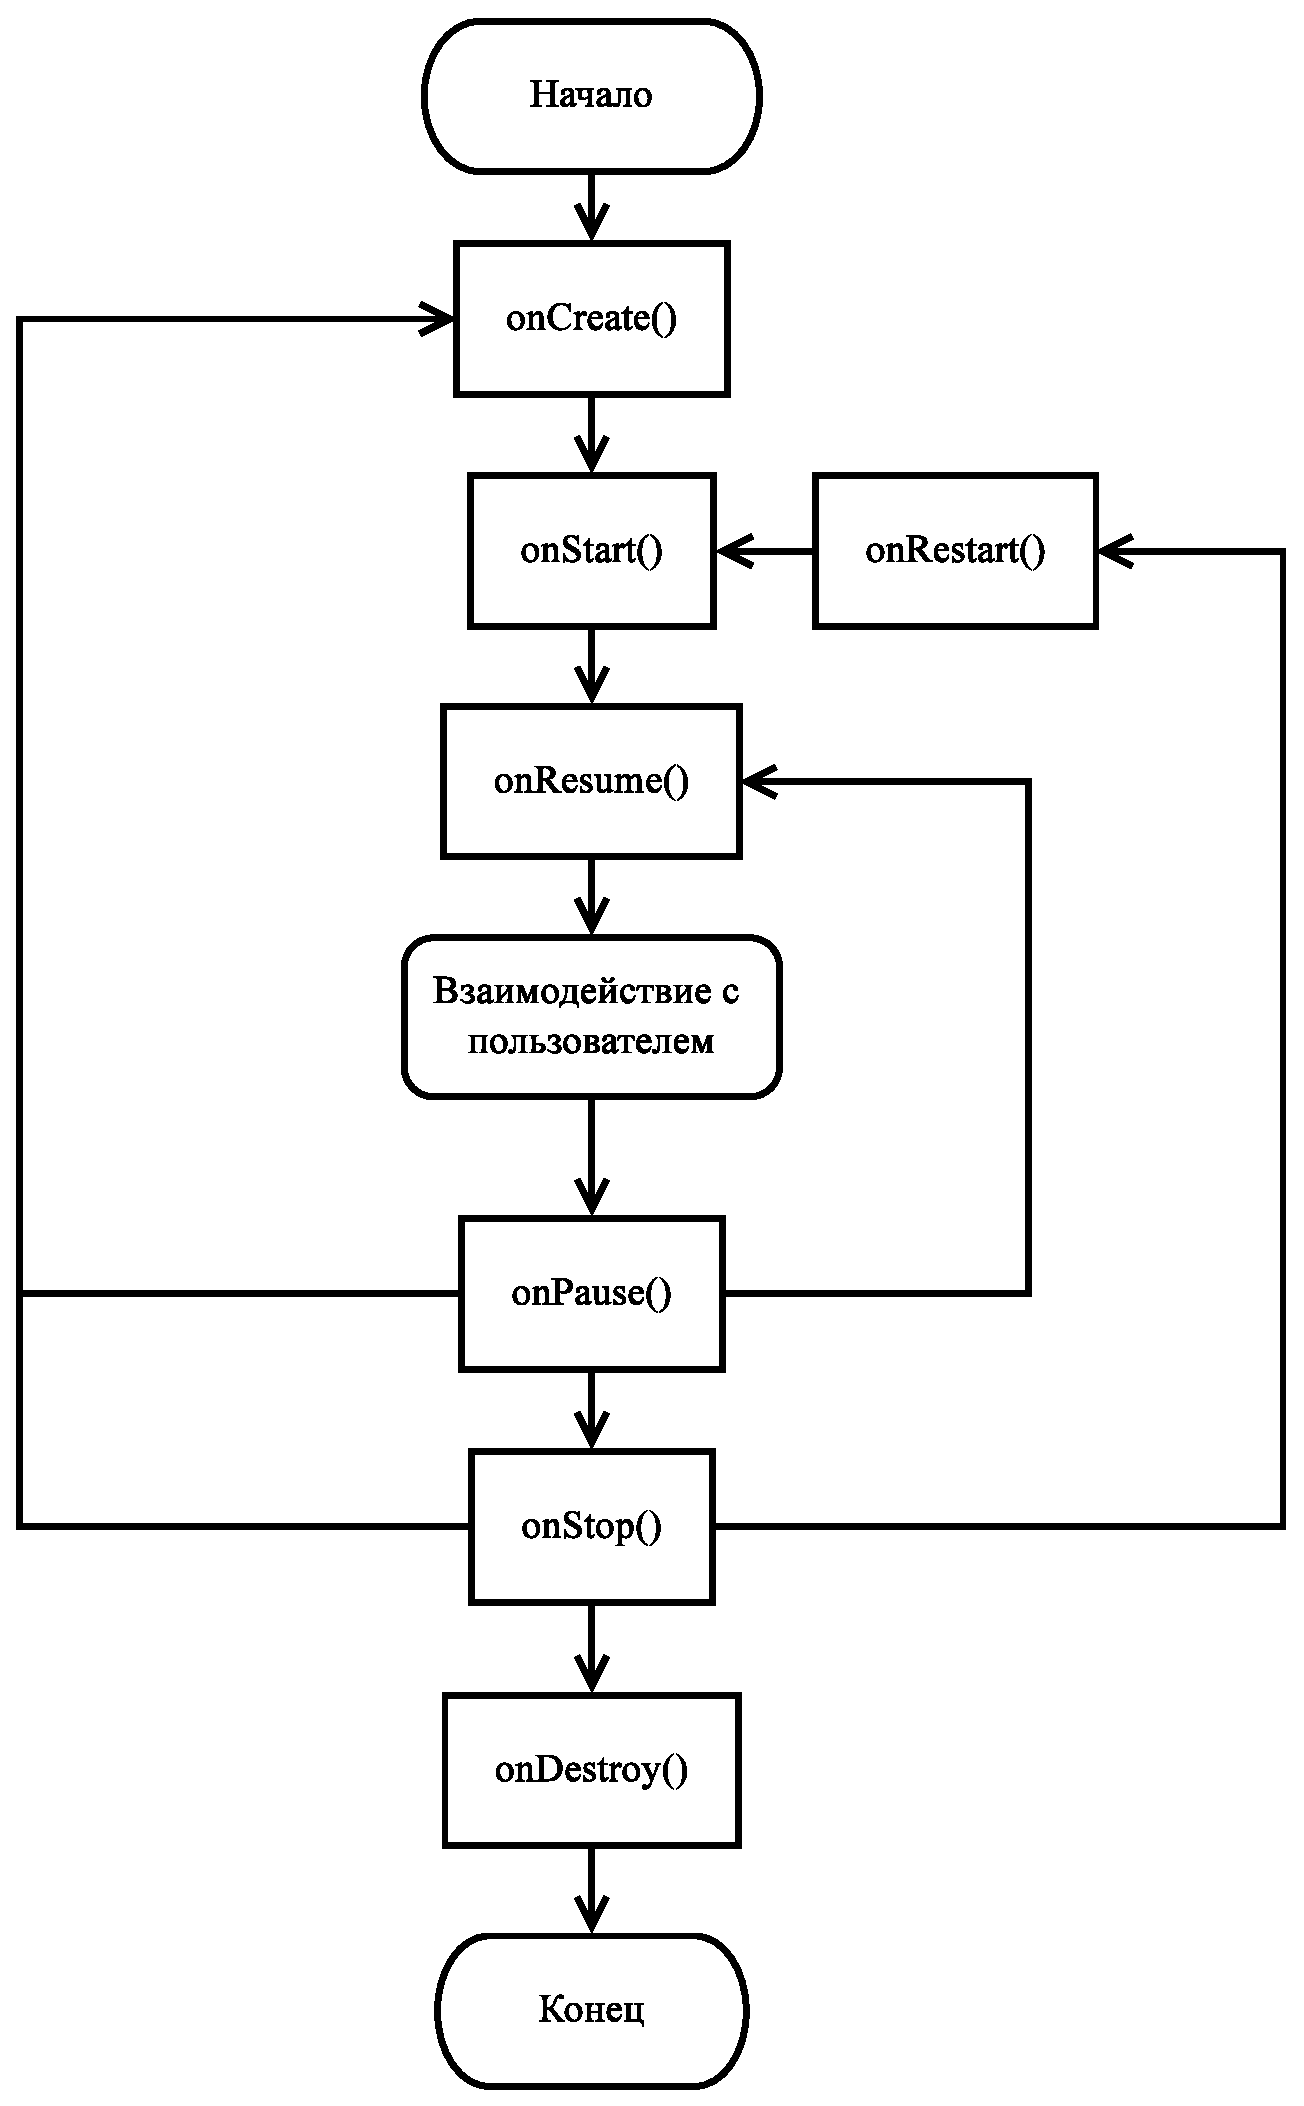
\includegraphics[height=30cm]{fig/implementation_ui_lifecycle_activity.eps}

    \vspace{2cm}
    {\Huge{Жизненный цикл экрана приложения}}
  \end{minipage}
\end{ESKDdrawing}

\setcounter{page}{1}
\ESKDthisStyle{formI}
\begin{ESKDdrawing}
\end{ESKDdrawing}

\end{document}
